\section{Introduction}\label{sec:intro}
% Problem, importantness, and specific question
Reward is a fundamental brain function that shapes our behavior through reward-based learning, or reinforcement learning (RL). Positive rewards encourage us to eat food and find mating partners, while negative rewards, such as pain and fatigue, help us protect ourselves. However, regardless of its importantness to animal lives, the evolutionary process of such rewards system is underexplored. Reward signals should have evolved to help animals survive and reproduce offspring (e.g., by~\cite{schultzNeuronalRewardDecision2015}), but what kind of environmental conditions has influenced the evolution of varieties of rewards remains unclear.

% What we do
While biological studies in evolution are important, the difficulty of observing reward evolution in real animals motivates us the use of artificial evolutionary simulation. Hence, we conduct an evolutionary simulation of RL agents to examine how different environmental conditions lead to different rewards. Each agent inherits a reward function from its parent and learns to get more rewards by RL during its lifetime. Contrary to previous studies on the evolution of learning \citep{hintonHowLearningCan1987,singhWhereRewardsCome2009} with centralized selection strategies, we design a distributed evolutionary model inspired by embodied evolution (EE) framework \citep{watsonEmbodiedEvolutionDistributing2002,bredecheEmbodiedEvolutionCollective2018}. In our model, birth and death for agents are evaluated independently based on their age and internal energy level, allowing the population change. With this approach, we expect that rewards contributing to population growth is selected.

% Simulation
We implement our distributed evolution framework based on 2D physics simulation using JAX \citep{jax2018github} to accelerate simulation by GPU. In this environment, we let agents to evolve simple reward functions that map food intake and the magnitude of motor output to scalar, which we expect to correspond to food pleasure and fatigue. Our results show that biologically reasonable reward functions evolve from randomly initialized ones given sufficient learning ability. We further find that metabolic balance, food density, and movement of food locations influence the shape of reward function.

\section{Preliminaries and Related Works}\label{sec:related}
We follow the standard computational RL framework \citep{suttonReinforcementLearningIntroduction2018} based on the Markov decision process (MDP). MDP $\M{}$ consists of a tuple $(\X{}, \A{}, p, r, \gamma)$, where $\X{}$ is reward function, and $\gamma \in [0, 1]$ is the discount factor. A standard objective in MDP is the discounted cumulative return $G \defequal{} \sum_{t=0}^{\infty}\gamma^t R_{t}$, where $R_t$ is the reward received at time $t$. An RL agent has policy $\pi: \X \times \A \rightarrow [0, 1]$ and seeks to find the the optimal policy $\pi^{*}$ that maximizes $\E \left[G|\pi\right]$. The state-value function $V^\pi(s) \defequal \sum_{a \in \A} \pi(a|s) \left( r(s, a) + \gamma \sum_{s' \in \X} P(s'|s, a) V^\pi(s') \right)$ is often used in RL algorithms. Observation $o \in \Omega~(\Omega \subseteq \X)$ refers to a part of the state that an agent can observe.

Our reward model is inspired by the neuroscience of reward system \citep{schultzNeuronalRewardDecision2015, berridgePleasureSystemsBrain2015}. Notably, \citet{berridgeDissectingComponentsReward2009} argue that the brain reward system consists of three independent components: liking, wanting, and learning. In analogy with computational RL, liking corresponds to reward function, wanting corresponds to learned policy, and learning corresponds to learning state value $V$.

While there were previous attempts to evolve rewards in a single-agent setting \citep{singhWhereRewardsCome2009,niekumEvolutionRewardFunctions2011,zhengWhatCanLearned2020},
%While evolutionary robotics studies \citep{nolfiEvolutionaryRoboticsBiology2004} often employ a centralized selection scheme similar to genetic algorithm \citep{mitchellIntroductionGeneticAlgorithms1998},
%where highly evaluated elites are selected as parents. On the contrary,
we empoloy a distributed embodied evolution (EE) framework \citep{watsonEmbodiedEvolutionDistributing2002,bredecheEmbodiedEvolutionCollective2018}
%that employs a decentralized evolution without centralized evaluation
where agents evolve locally following birth and death rules. This method has the advantage that the evaluation of genetic traits depends on population dynamics, which is more natural.

Our work is inspired by the series of studies \citep{elfwingBiologicallyInspiredEmbodied2005,elfwingDarwinianEmbodiedEvolution2011,elfwingEmergencePolymorphicMating2014}, which tried to evolve parameters related to RL through EE framework. Notably, \citet{elfwingDarwinianEmbodiedEvolution2011} evolved supplementary sharing rewards and parameters of RL agents.
Inspired by these works, we attempt to evolve the entire reward functions in our experiments.

\section{Simulation Model and Environment}\label{sec:method}

\begin{figure}[t]
  \centering{}
  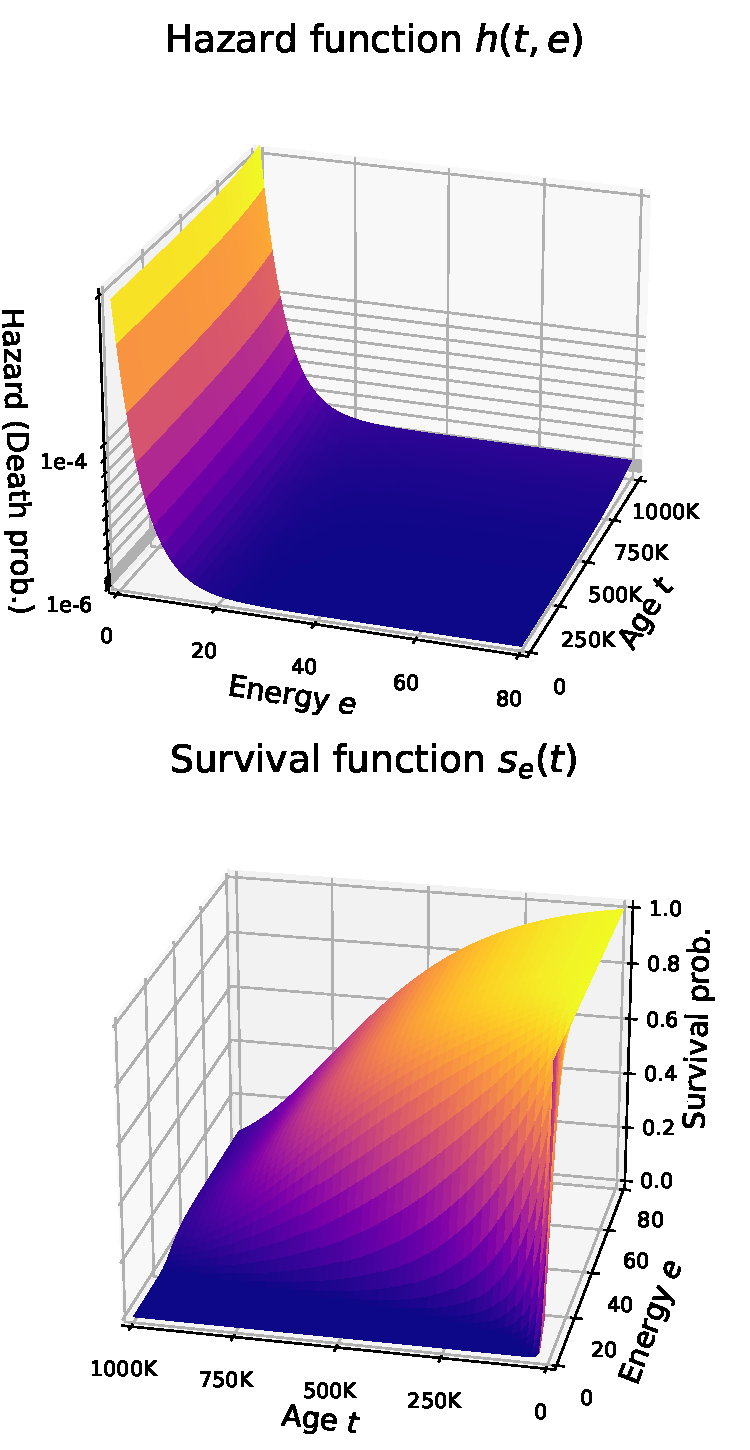
\includegraphics[width=6cm]{hazard_and_survival.pdf}
  \caption{
    \textbf{Upper:} Hazard function $h(t)$ used in our experiments.
    \textbf{Lower:} Survival function $S(t)$ corresponding to the hazard function above.
  }\label{figure:hs}
\end{figure}

\paragraph{Energy-based death and birth model}
We employ an energy-based metabolic model similar to \citet{hamonEcoevolutionaryDynamicsNonepisodic2023}. Each agent maintains their energy level $e$, which increases by eating food and decreases by the basal metabolism and taking a motor action.
The mortality of an agent with energy level $e$ and age $t$ is modeled by the hazard function:
\begin{align}
  h(t, e) = \frac{\kappa_{h}}{1 + \alpha_{e}\exp(\beta_{he}e)} + \alpha_{t} \exp(\beta_{ht} t).
  \label{eq:h}
\end{align}
The first term in \cref{eq:h} increases as energy levels decrease following a sigmoidal curve where $\kappa_{h}$ is the scale, $\beta_{he}$ is the slope, and $\alpha_{e}$ defines the shape when $e=0$. The latter term increases exponentially as the agent ages with the cale $\alpha_{t}$ and the slope $\beta_{ht}$, called Gompertz hazard model \citep{gompertzXXIVNatureFunction1825,kirkwoodDecipheringDeathCommentary2015}.
We show the shape of $h$ with parameters used in our experiments in the upper panel in \cref{figure:hs}. The lower panel in \Cref{figure:hs} shows the survival function $s_{e}(t) = \exp (-\int_{0}^{t}(h(t, e)) dt)$ corresponding to $h$, which is the probability for an agent to survive to the age $t$ under the assumption that it keeps the same energy level $e$. We can see that the survival probability more sharply decays with aging when the energy level is low.

\begin{figure}[t]
  \centering{}
  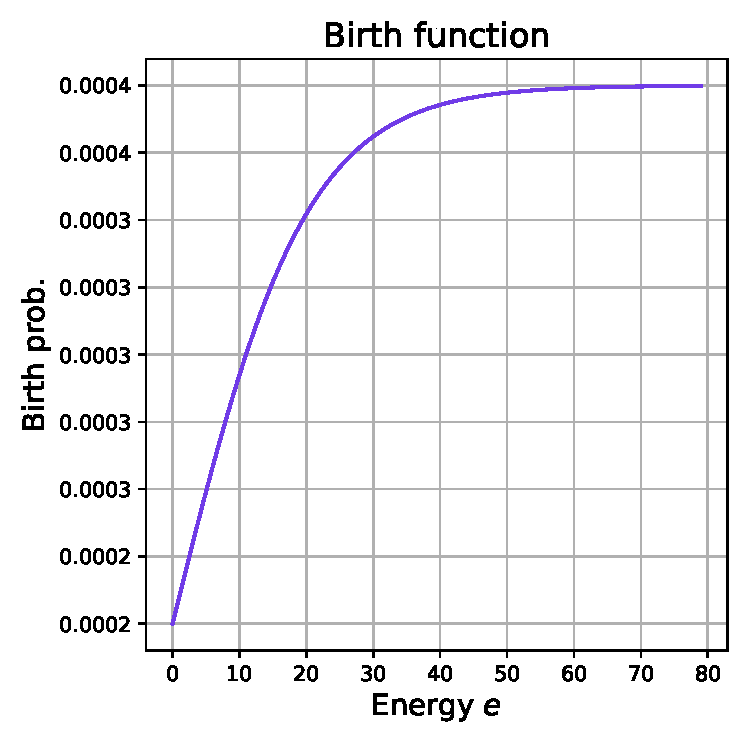
\includegraphics[width=6cm]{birth.pdf}
  \caption{Birth function $b(e)$ used in our experiments.}\label{figure:birth}
\end{figure}

\begin{table}[t]
  \begin{subtable}[h]{0.45\columnwidth}
    \centering
    \begin{tabular}{cc}
      \toprule
      Parameter & Value \\
      \midrule
      $\kappa_{h}$ & 0.01 \\
      $\alpha_{e}$ & 0.02 \\
      $\beta_{he}$ & 0.2 \\
      $\alpha_{ht}$ & \num{2e-7} \\
      $\beta_{t}$ & \num{4e-6} \\
      \bottomrule
    \end{tabular}
  \end{subtable}
  \begin{subtable}[h]{0.45\columnwidth}
    \centering
    \begin{tabular}{cc}
      \toprule
      Parameter & Value \\
      \midrule
      $\kappa_{b}$ & \num{4e-4} \\
      $\beta_{b}$ & 0.1 \\
      \bottomrule
    \end{tabular}
  \end{subtable}
  \caption{Parameters of $h$ (left) and $b$ (right) used in our experiments.}\label{table:hb}
\end{table}

For simplicity, we employ an asexual reproduction model with the birth function, the probability for an agent with energy level $e$ to produce a child in a time step:
\begin{align}
 b(e) &= \frac{\kappa_{b}}{1 + \exp(\beta_{b}e)}.
 \label{eq:b}
\end{align}
The birth rate $b(e)$ increases with $e$ following a sigmoidal curve where $\kappa_{b}$ is the scale and $\beta_{b}$ is the slope.
\Cref{figure:birth} shows the shape of $b$ for the parameters used in our experiments. We show all paramters of $h$ and $b$ in \cref{table:hb}. With this choice of paramters, we exepect the maximum liftime of an agent is around \num{1e6} steps.

\paragraph{Environment}

\begin{figure}[t]
  \centering
  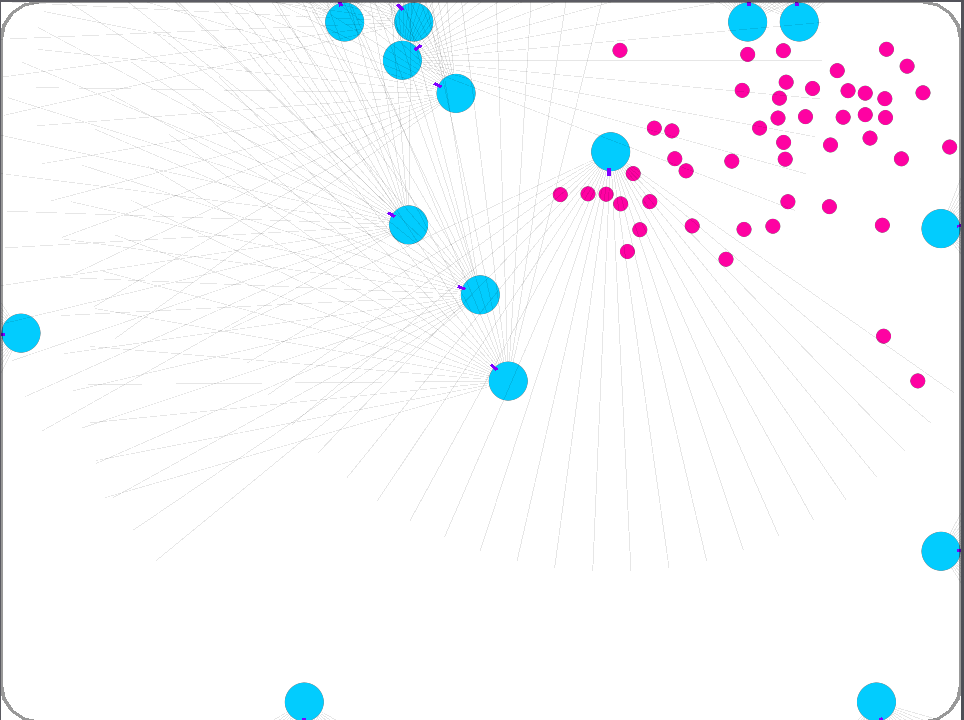
\includegraphics[width=6cm]{emevo-ss.png}
  \caption{
    Simulation environment used in our experiments.
    Blue circles are agents, red circles are foods, and outer gray lines are walls.
    Thin gray lines around agents indicate distance sensors.
  }\label{figure:env}
\end{figure}

\begin{figure}[t]
  \begin{subfigure}[t]{4cm}
    \centering
    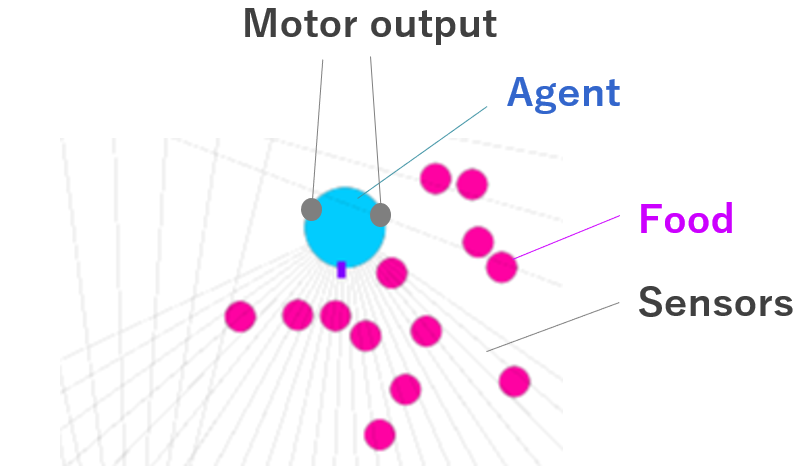
\includegraphics[width=4cm]{emevo-anno.png}
  \end{subfigure}
  \begin{subfigure}[t]{4cm}
    \centering
    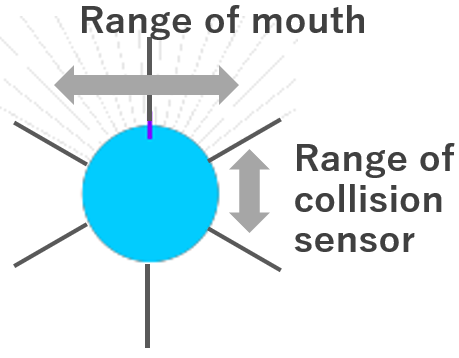
\includegraphics[width=4cm]{emevo-mouth.png}
  \end{subfigure}
  \caption{
    Description of the environment.
    The left figure shows an agent, foods, distance sensors, and the positions of motor outputs.
    The right figure shows the ranges of an agent's mouth and each collision sensor.
  }\label{figure:env-discr}
\end{figure}

We designed a continuous 2D environment shown in \cref{figure:env}. Blue circles indicate agents and red circles indicate foods. The environment is implemented by a 2D rigid-body physics simulation. Agents can move by producing driving forces on the left and right sides of the body, as shown in \cref{figure:env-discr}. An agent has multiple range sensors in its front, which can sense the type and the distance to the closest object within $120$ degree. Sensible objects include foods, other agents, and walls. They can also sense the collision with each object and the approximate location of the collision with a resolution of $60$ degree, as shown in \cref{figure:env-discr}.

% This eat-driven emergence is not consistent with the growth model below. Better report the actual food producing process rather than theoretical approximation.
An agent can eat food by touching it and gain energy $e_{\mathrm{food}}$. After foods are eaten, they are regenerated in a random place. To regulate the rate of food regeneration, we maintain the internal food number $n_{t}$ at time $t$ which follows a logistic growth function: $n_{t + 1} = n_{t} + gn_{t}(1 - \frac{n_{t}}{n_{\mathrm{max}}}) - n_{t}^{\mathrm{eaten}}$, where $g$ is the growth rate, $n_{\mathrm{max}}$ is the capacity of food, and $n_{t}^{\mathrm{eaten}}$ is the number of eaten foods at time $t$. Food is regenerated when the integer part of $n^{t}$ is more than the actual number of foods in the environment. We use $e_{\mathrm{food}} = 1$ in our experiments. In experiments with less nutrient-poor or poisonous foods, they have different energy gain $e_{\mathrm{poor}} = 0.2$ and $e_{\mathrm{poison}} = -0.2$.

When an agent makes a child, a new agent is placed in a random location sampled from a Gaussian distribution centered around its parent. Reproduction fails when all $10$ sampled locations are not available. The child inherits a proportion of the parent's energy $\eta e \in [0, 1]$, and the parent's energy level decreases to $(1-\eta)e$, where $\eta \in [0, 1]$ is the ratio of energy sharing. We used $\eta = 0.4$ in our experiments. The child also inherits its reward function from the parent with some mutation.

Since we need to maintain agents for evolution, the multi-agent interaction can be a huge bottoleneck in our simulation. To overcome this challenge, we implement our environment using JAX Python library \citep{jax2018github} so that the entire simulation loop is executed on GPU. Inspired by recent works on 3D rigid body physics simulation using JAX (e.g., \citet{brax2021github} and MuJoCo \citep{todorov2012mujoco} MJX\footnote{\url{https://mujoco.readthedocs.io/en/stable/mjx.html}}), we implement our 2D physics engine using JAX and build our
environment on top of that, optimizing it for multi-agent setting. Our simulator implements projected Gauss-Seidel method with position correction \citep{catto2005iterative} that is pretty common in 2D game physics engines such as Box2D\footnote{\url{https://box2d.org}} and Chipmunk\footnote{\url{https://chipmunk-physics.net}}.

\paragraph{Reward Function with Evolving Weights}
We assume that the reward function is determined at birth with mutation and does not change during an agent's lifetime. We use food intake and the magnitude of the agent's action (motor output) as inputs to the reward function. We expect a positive food reward evolve to acquire energy and a negative reward for action evolve to save energy.
We model the reward of an agent $i$ at time $t$ by $r^{i}_{t} = w_{\mathrm{food}}^{i}n_{t}^{i} + c_{\mathrm{act}} w_{\mathrm{act}}^{i}|a_{t}^{i}|$, where $n_{t}^{i}$ is the number of foods that the agent ate and $|a_{t}^{i}|$ is the Euclid norm of the agent's motor output. $w_{\mathrm{food}}^{i}$ and $w_{\mathrm{act}}^{i}$ are evolvable reward parameters of an agent $i$. Because an agent gets the action reward at every step while it doesn't get the food reward so often, we use a fixed parameter $c_{\mathrm{act}}$ to scale the action reward. We use $c_{\mathrm{act}} = 0.01$ in our experiments. In experiments with poor or poisonous foods, we use another evolvable reward parameter $w_{\mathrm{poor}}^{i}$ or $w_{\mathrm{poison}}^{i}$.

\paragraph{Reinforcement Learning}
We use Proximal Policy Optimization \citep{schulmanProximalPolicyOptimization2017} as an RL algorithm because of its fast computation time. In addition to the touch and collision sensor inputs in \cref{figure:env-discr}, an agent takes its angle, velocity, and energy level as an observation. The action space is a continuous two-dimensional vector $\mathbf{a} = (f_{\mathrm{left}}, f_{\mathrm{right}})$, where $f_{\mathrm{left}}$ and $f_{\mathrm{right}}$ are the forces applied to the left and right sides of the body. The agent's policy is represented by a multi-layer perceptron with hyperbolic tangent activation, similar to the one used in continuous control experiments in \citep{schulmanProximalPolicyOptimization2017}.

\begin{table}[t]
  \centering
  \caption{RL parameters}\label{tab:rl-param}
  \begin{tabular}{ll}
    \toprule
    Paremeter & Value \\
    \midrule
    Discount factor ($\gamma$) & 0.999 \\
    Rollout steps ($N$) & 1024 \\
    Minibatch size & 256 \\
    Number of optimization epochs & 10 \\
    PPO Clipping parameter & 0.2 \\
    Entropy coeff. & 0.0 \\
    GAE parameter ($\gamma$) & 0.95 \\
    Adam learning rate & \num{3e-4} \\
    Adam $\epsilon$ & \num{1e-7} \\
    \bottomrule
  \end{tabular}
\end{table}

% Add a line for reward acquisition; after observation or action?
\begin{algorithm}[t]
  \caption{Reward evolution with asexual reproduction}\label{alg:reward-evo}
  \begin{tabular}{lll}
    \textbf{Input:} & $Pop$ & Initial population of agents \\
                    & $Env$ & Simulation environment \\
                    & $h, b$ & Hazard and birth functions \\
                    & $m$ & mutation function \\
                    & $N$ & Rollout step used in RL \\
                    & $\eta$ & Energy share ratio
  \end{tabular}
  \begin{algorithmic}[1]
    \Loop{}
    \LComment{Interact with environment}
    \ForAll{$agent \in Pop$}
      \State{$o \gets agent$'s observation in $Env$}
      \State{$a \gets $ sample from $agents$'s policy $\pi_{agent}(\cdot|o)$}
      \Once{in $N$ steps}
        \State{Update $agent$'s policy $\pi_{agent}$ via RL}
      \EndOnce{}
    \EndFor{}
    \State{Step $Env$ using collected actions}
    \State{Update $agent$'s energy level}
    \LComment{Process birth and death}
    \ForAll{$agent \in Pop$ with energy $e$ and age $t$}
      \State{$e \gets e + e_{\mathrm{food}} n_{\mathrm{food}} - |a|$}
      \With{Probability $b(e)$} \Comment{Birth}
        \State{$e \gets (1 - \eta) e$}
        \State{$r \gets agent$'s reward function}
        \State{Create a new agent with $\eta e$ and $m(r)$}
      \EndWith{}
      \With{Probability $h(t, e)$} \Comment{Death}
        \State{$agent$ is removed from $Pop$ and $Env$}
      \EndWith{}
    \EndFor{}
  \EndLoop{}
\end{algorithmic}
\end{algorithm}

\paragraph{Simulation Procedure}
We show the pseudocode of our entire simulation procedure in \cref{alg:reward-evo}. Each agent has its innate, immutable reward function and learnable neural network policy. At each step, it observes sensory inputs from the environment and takes action. Once in $N$ steps, the agent updates its policy via RL using the past $N$ step experiences. After environmental interaction, all agents can make a child and die based on the birth function $b$ and hazard function $h$. The new agent inherits a fraction of the parent's energy and mutated reward function. As mutation, we add uniform noise to each $s$ and $w$ with probability $0.4$. We show some relevant parameters in \cref{ap:param}.

\section{Results}

As a baseline environment, we use the setting where food is always regenerated in the upper right of the room, as the left figure in \Cref{figure:env} shows. In this environment, we tuned environmental parameters (e.g., maximum number of foods and growth rate) to stabilize the population around $100$. We show all environmental parameters in \cref{ap:param}. All experiments start with $50$ agents that have energy level $40.0$ and randomly initialized reward weights. We conducted \num{1e7} step of the simulation, resulting from $300$ to $400$ generations, which takes $14\sim16$ hours on NVIDIA P100 GPUs.

\Cref{subfigure:bl} shows the evolved reward weights with 5 random seeds in the baseline environment. Surprisingly, the food reward weight is only stable positive for one random seed. It unstably goes up and down or stays negative in one random seed. On the contrary, reward weights for colliding with walls and other agents are stably negative, which is reasonable because sticking around walls is not good for foraging, and sticking to other agents might reduce the chance of making a child. The reward weight for action tends to be positive. This contradicts our expectations that it would evolve into negative, like fatigue.

To investigate the reason why the evolution of food reward can be unstable, we closely look at our simulation run with seed $5$, where food reward decreases. \Cref{subfigure:s5} shows the scatter plot of reward weights in this run from \num{4e6} to \num{9e6} steps, where blue color indicates smaller food rewards and red color indicates larger. We can see a tendency that agents with lower food rewards tend to have higher wall and action rewards, which is reasonable because both sticking around walls and just moving can help foraging. On the contrary, we can see two different modes in agent and action rewards. In the medium of \cref{subfigure:s5} (between \num{6e6} and \num{7e6} steps), agents with smaller rewards tend to have smaller negative rewards for colliding with an agent, while they tend to have larger agent rewards later. On the contrary, in the case where the food reward remains stable, shown in \cref{subfigure:s2} (seed $2$), the magnitude of other collision rewards (agent and wall) is relatively small, and they don't look have a large effect. The reward for action increases over the course of evolution, which might help foraging with food rewards.

To investigate the difference in the two cases, we focus on the period we filled orange in the first row of \cref{subfigure:s5} and \cref{subfigure:s2}, where both negative and positive food rewards coexist. We plot agents' life history in this period in \cref{figure:s5lh}, where thin lines show the agents' trajectories, dots show places where agents got children, and different colors correspond to the value of food rewards. In both figures, we can see that agents' trajectories are concentrated around the food location, while they make children in more distributed places because of the environmental constraint that makes it more difficult to have a child in a crowded area.
Although we don't see significant differences in agents' trajectories, we can see a tendency that agents with negative food rewards are distributed more distant from the food rewards because of the smaller negative food reward in \cref{subfigure:s2lh}. On the contrary, we guess that relatively larger negative food rewards in \cref{subfigure:s5lh} are not very harmful, especially with stronger rewards for collision with agents and walls. Instead, it looks like the negative rewards for colliding each other helps agents to form a collective behavior that doesn't look very directed.


In the baseline environment, agents are densely located in the food location, which seems to influence the evolution of rewards. For example, negative rewards for food or another agent would help them move to sparser locations where they are more likely to produce offspring. Therefore, we conduct another experiment with more distributed food regeneration (\texttt{spread foods} in the figure) and moving food location after eating $1000$ foods (\texttt{food reloc.} in the figure). \Cref{subfigure:blcomp} compares the evolved reward functions with the baseline. To make the comparison easier, we average the reward weight of all available agent at a certain step, and plot the mean for $5$ runs each. Although food rewards can be unstable with all these three settings, the \texttt{spread foods} setting is the most stable in the sense that food reward is stable in 3 runs within 5 random seeds. Reward weights for colliding with walls and other agents are almost always negative, as in the baseline setting. The reward for action is generally positive, but sometimes goes negative with \texttt{spread foods} setting, producing the population that sticks to the wall.

\section{Conclusion}
In this paper, we propose a distributed evolutionary simulation to investigate the evolution of reward function. Our simulation results show that the evolution of food reward is often unstable under many conditions because of food regeneration and spatial constraints. We show that the sparseness of the population and foods can be an important factor in the evolution of stable food rewards.